\documentclass[11pt,notitlepage]{article}
\usepackage{amsfonts, amsmath, amssymb, amsthm,fullpage,mdwlist,graphicx,cancel}
\setlength{\textheight}{9.25in}
\setlength{\textwidth}{6.5in}
\setlength{\topmargin}{0.0in}
\setlength{\headheight}{0.0in}
\setlength{\headsep}{0.0in}
\setlength{\leftmargin}{0.0in}
\setlength{\oddsidemargin}{0.0in}
\setlength{\parindent}{0pc}
\everymath{\displaystyle}
\DeclareMathOperator*{\res}{Res} 
\newtheorem{thm}{Theorem}[section]
\newtheorem{exc}{Exercise}[section]
\title{$\mathbb{C}$alculus of Residues}
\author{Anish Tondwalkar}
\date{April Fools' 2011}
\begin{document}
\begin{center}
\Large{$\mathbb{C}$alculus of Residues}
\par
\large{Anish Tondwalkar}
\par
\small{April Fools' 2011}
\end{center}
Residue theory is a powerful tool to kill some integrals.  I have a proof and a little analysis in here, but I left most of them as exercises for you to do on your own.  To properly develop the theory we need some other stuff first \ldots
\section{Complex Integrals}
Since in the complex plane, we're now on a plane, not a line, there's more than one way to get from one point to another. Therefore, most the integrals you see during this lecture are contour integrals. We define an integral along some path in $\mathbb{C}$ the same way we do in multivar for $\mathbb{R}^2$. One really trivial thing you should realize is that:
\begin{thm}[Cauchy's Integral Theorem]
$\oint_C f(z) dz = 0$ 
\end{thm}
\begin{flushright}
if $f$ is analytic (a.k.a.\! conservative) inside $C$ and continuous on $C$.
\end{flushright}
\begin{exc}
Prove this. Hint: Plug in real and imaginary parts into Laplace's Equation ($\nabla^2f=0$), in order to obtain the Cauchy-Riemann equations. 
\end{exc}
\section{Cauchy's Integral Formula}
\begin{thm}[Cauchy's Integral Formula]
$\oint_C \frac{f(z)}{z-z_0} dz = 2\pi i f(z_0)$ 
\end{thm}
\begin{flushright}
if $f$ is analytic inside $C$.
\end{flushright}
\begin{proof}

Start with this contour, split as so:
$$\tilde C = C - C_\epsilon +\cancel{C_{+} + C_{-}}$$
\center{
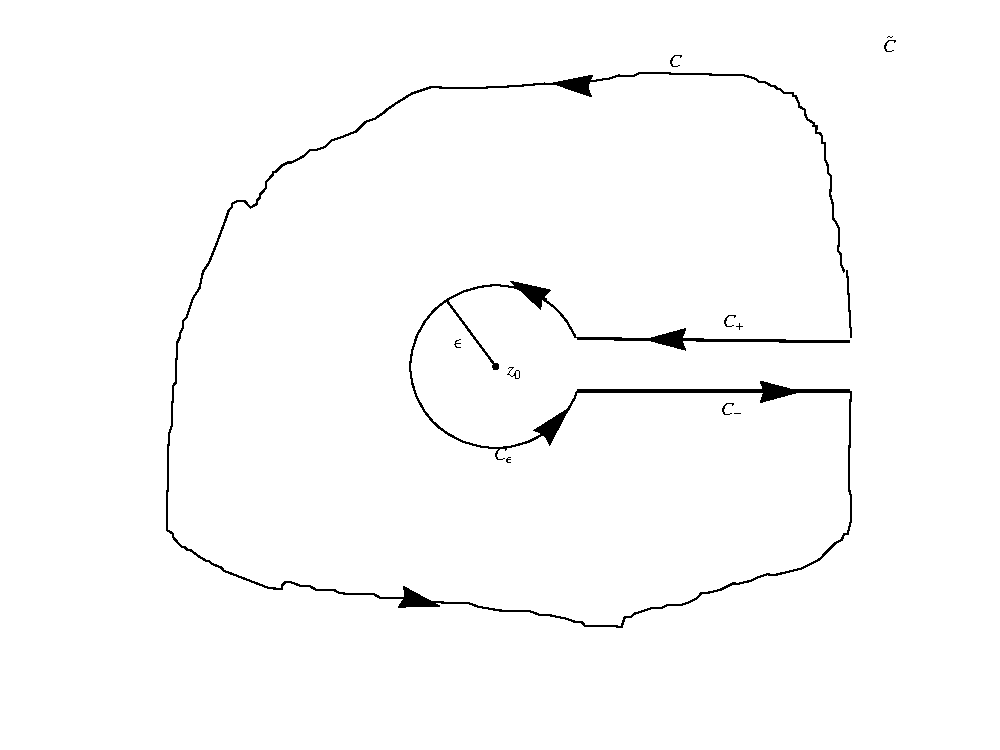
\includegraphics[scale=.3]{ctwiddle}
}
$$\oint_{\tilde C} \frac{f(z) dz}{z-z_0} 
= 0 
=\oint_{ C} \frac{f(z) dz}{z-z_0} -\oint_{C_\epsilon} \frac{f(z) dz}{z-z_0}$$
$$\oint_{C} \frac{f(z) dz}{z-z_0} 
= \oint_{C_\epsilon} \frac{f(z) dz}{z-z_0}
= \oint_{C_\epsilon} \frac{f(z_0 + \epsilon e^{i\theta}) }{\epsilon e^{i\theta}} \epsilon i e^{i\theta} d\theta 
= i \int_0^{2\pi} f(z_0 + \cancelto{0}{\epsilon e^{i\theta}}) d\theta \rightarrow 2\pi i f(z_0) $$
\end{proof}
Note that for this to hold, $f$ has to be analytic, but not necessarily at $z_0$
\section{Laurent Series}
Now we can find something interesting if we try to develop Taylor Series using this fact, so let's do it! Let $t$ on some arbitrary $C$. We're looking for an expansion in powers of $(z-a)$, with $a$ inside $C$. 
$$ f(z) = \frac1{2\pi i}\oint_{C} \frac{f(t) dt}{t-z} $$
$$\frac1{t-z} = \frac1{(t-a)-(z-a)} = \frac1{t-a}\frac1{1-{\frac{z-a}{t-a}}} = \frac1{t-a}\sum_{n=0}^\infty\left(\frac{z-a}{t-a}\right)^n $$
$$ f(z) = \frac1{2\pi i}\oint_{C} \frac{f(t) dt}{t-a} \sum_{n=0}^\infty\left(\frac{z-a}{t-a}\right)^n  = \frac1{2\pi i} \sum_{n=0}^\infty{(z-a)}^n \oint_{C} \frac{f(t) dt}{(t-a)^{n+1}} $$
Now, if we write $f(z) = \sum_{n=-\infty}^\infty A_n (z-a)^n$, we arrive at the nice results:
 $$f^{(n)}(a) = n! A_n$$
 $$A_n = \frac1{n!2\pi i} \oint_{C}\frac{f(t) dt}{(t-a)^{n+1}}$$
We've proved this for positive n, but not for negative n. That proof is left as an exercise.
Since we also have negative powers of n, this expansion also works for functions that are not analytic, specifically, functions whose discontinuity is classified as a pole. The order of this pole is the lowest n for which $A_n \not=0$ in the expansion. A pole of order $1$ is also called a simple pole. Furthermore, the residue is defined, $$\res_{z=a} f(z) = A_{-1}$$
\section{Residues}
Here are three theorems that are useful and easy to prove:
\begin{thm}[Residues for simple poles]
If $f(z)=\frac{g(z)}{h(z)}$, $h(z_0)=0$, $h'(z_0)\not=0$, then $$\res_{z=z_0} f(z) = \frac{g(z_0)}{h'(z_0)}$$
\end{thm}
\begin{thm}[Residues for poles of higher order]
If $z_0$ is an $m^{th}$ order pole, 
$$\res_{z=z_0} f(z) = \lim_{z\rightarrow z_0} \frac1{(m-1)!} D_z^{m-1} \left[(z-z_0)^m f(z)\right]$$
\end{thm}
\begin{thm}[Cauchy's Residue Theorem]
If $f$ has isolated poles at $z_0,z_1,z_2, \ldots z_k$ inside $C$, and in analytic elsewhere inside $C$,
$$\oint_C f(z) dz = 2\pi i\sum_{i=0}^k \res_{z=z_i} f(z)$$
\end{thm}
\begin{exc} Prove these
\end{exc}
Now that we can do integrals on contours in the complex plane, we can use them to evaluate real definite integrals. Finally, some more applied stuff.
\section{Evaluation of Real Definite Integrals}
Let's use this to find $$\int_{-\infty}^{\infty} \frac{\cos(x)dx}{z^2+1}$$
First note: $$\int_{-\infty}^{\infty} \frac{\cos(x)dx}{z^2+1} = \Re\left[\int_{-\infty}^{\infty} \frac{e^{iz}dx}{(z-i)(z+i)}\right]$$
So we use this contour: $$C = \cancelto0{C_\infty} + C_0$$
%\includegraphics{up}


\end{document}
